%\documentclass[show notes]{beamer}       % print frame + notes

\documentclass[11pt,handout]{beamer}   % only notes
%\documentclass[aspectratio=169]{beamer}              % only frames
\usefonttheme[onlymath]{serif}
\definecolor{DarkGray}{HTML}{63656a}
\setbeamertemplate{note page}[plain]
\setbeamertemplate{navigation symbols}{}
\setbeamertemplate{footline}[text line]{%
  \hfill\strut{\scriptsize\sf\color{DarkGray}\today}\hfill\strut{%
        \scriptsize\sf\color{DarkGray}%
        \quad\insertframenumber/\inserttotalframenumber
    }%
}

\usepackage{amsfonts}


\beamertemplatenavigationsymbolsempty


\title[Your Short Title]{Nonlinear Control Systems}
\subtitle{Lsn 3: Fundamentals of Lyapunov Theory}
\author{I. Weintraub, Dr. Cobb, \& Capt. Hess}
\institute{Air Force Institute of Technology}
\date{\today}

\begin{document}

\begin{frame}
  \titlepage
\end{frame}

\begin{frame}
\frametitle{Nonlinear Systems and Equilibrium Points}
\small
\textbf{Nonlinear Systems}\\
A \underline{nonlinear dynamic system} can usually be represented by a set of nonlinear differential equations in the form:
\begin{equation*}
\dot{\mathbf{x}} = \mathbf{f}(\mathbf{x},t)
\end{equation*}
where $\mathbf{f}$ is an $n \times 1$ nonlinear vector function, and $\mathbf{x}$ is the $n \times 1$ state vector. We define $n$ as the \textit{order} of the system. If we define the control $\mathbf{u}(t)$ as the control input. If the plant dynamics are:
\begin{equation*}
\dot{\mathbf{x}} = \mathbf{f}(\mathbf{x},\mathbf{u},t)
\end{equation*}
And some control law has been selected
\begin{equation*}
\mathbf{u} = \mathbf{g}(\mathbf{x},t)
\end{equation*}
then the closed-loop dynamics are
\begin{equation*}
\dot{\mathbf{x}} = \mathbf{f}(\mathbf{x},\mathbf{g}(\mathbf{x},t),t)
\end{equation*}
A special class of system is the linear system. The general form of the dynamics are of the form:
\begin{equation*}
\dot{\mathbf{x}} = \mathbf{A}\mathbf{x}
\end{equation*}
\end{frame}

\begin{frame}
\frametitle{Nonlinear Systems and Equilibrium Points}
\small
\textbf{Autonomous and Non-Autonomous Systems}\\
The \textit{nonlinear system} is said to be \underline{autonomous} if $\mathbf{f}$ \textit{does not depend explicitly on time, i.e.,} if the systems state equation can be written
\begin{equation*}
\dot{\mathbf{x}} = \mathbf{f(\mathbf{x})}
\end{equation*}
\textit{Otherwise the system is called \underline{non-autonomous}}\\
\vspace{6pt}
\textbf{Fundamental Difference:}\\
The fundamental difference between autonomous and non-autonomous systems lies in the fact that the state trajectory of an autonomous system is independent of the initial time, while that of a non-autonomous system generally is not.\\
\vspace{6pt}
\textbf{Examples:}\\
\begin{center}
$\dot{\begin{bmatrix}
x_1 \\ x_2
\end{bmatrix}} = \begin{bmatrix}
\cos(x_1) \\ \sin(x_2)
\end{bmatrix}$ Autonomous\\
\vspace{6pt}
$\dot{\begin{bmatrix}
x_1 \\ x_2
\end{bmatrix}} = \begin{bmatrix}
t \cos(x_1) \\ t \sin(x_2)
\end{bmatrix}$ Non-Autonomous\\
\end{center}
\end{frame}

\begin{frame}
\frametitle{Nonlinear Systems and Equilibrium Points}
\small
\textbf{Equilibrium Point}\\
\textit{A state $\mathbf{x}^*$ is an \underline{equilibrium point} of the system if once $\mathbf{x}(t)$ is equal to $\mathbf{x}^*$, it remains equal to $\mathbf{x}^*$ for all future time}.\\
\vspace{6pt}
Solving the autonomous system for the equilibrium state can be done by solving the system of equations represented by
\begin{equation*}
\mathbf{0} = \mathbf{f}(\mathbf{x}^*)
\end{equation*}
\textbf{Equilibrium Point for Linear Time-Invariant System}\\
A linear time-invariant system has a single equilibrium point (the origin $\mathbf{0}$) if $\mathbf{A}$ is nonsingular. If $\mathbf{A}$ is singular, it has an infinity of equilibrium points, which are contained in the null-space of the matrix $\mathbf{A}$. (i.e. the subspace defined by $\mathbf{Ax=0}$)\\
\vspace{6pt}
\end{frame}

\begin{frame}
\frametitle{Nonlinear Systems and Equilibrium Points}

\begin{columns}
\begin{column}{0.5\textwidth}
\textbf{Equilibrium Example:}\\
Pendulum with length $R$, mass $M$, drag $b$, and gravity $g$. State Space variables: $x_1 = \theta$ and $x_2 = \dot{\theta}$\\
\begin{equation*}
\frac{d}{dt}
\begin{bmatrix}
x_1\\x_2
\end{bmatrix} = \begin{bmatrix}
x_2\\\-\frac{b}{MR^2}x_2 - \frac{g}{R} \sin x_1
\end{bmatrix}
\end{equation*}
Equilibrium points given by:\\
\vspace{6pt}
$x_2 = 0$ and $\sin(x_1) = 0$ leading to points: $(0,0)$ and $(n\pi ,0)$
\end{column}
\begin{column}{0.5\textwidth}
\begin{center}
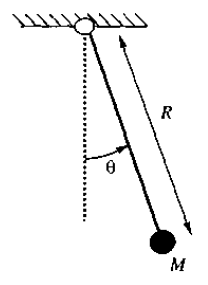
\includegraphics[width = 0.8\textwidth]{Figures/Fig31.PNG}
\end{center}
\end{column}
\end{columns}
\end{frame}

\begin{frame}
\frametitle{Equilibrium Example}
\small
\textbf{Known/Find/Given:}\\
Consider $\ddot{x} + (x-1)^4 \dot{x}^7 + x^5 = x^3\sin ^3(x)$
\begin{enumerate}
\item find the equilibrium points
\end{enumerate}
\textbf{Analysis:}\\
Let $x_1 = x$ and $x_2 = \dot{x}$. The state space representation is:
\begin{equation*}
\begin{aligned}
\dot{x}_1 &= x_2 = f_1(\mathbf{x})\\
\dot{x}_2 &= x_1^3sin^3(x_1) - x_1^5 - (x_1-1)^4x_2^7 = f_2(\mathbf{x})
\end{aligned}
\end{equation*}
Setting the R.H.S equal to zero to find the equilibrium points:
\begin{equation*}
\begin{aligned}
\dot{x_1} = 0 = f_1(\mathbf{x}_{eq}) = 0 &\Rightarrow x_{2} = 0\\
\dot{x_2} = 0 = f_2(\mathbf{x}_{eq}) = 0 &\Rightarrow 0 = x_1^3sin^3(x_1) - x_1^5 - (x_1-1)^4x_2^7
\end{aligned}
\end{equation*}
Plugging in $x_2 = 0$ we need to find the roots of the R.H.S in order to determine the equilibria.
\end{frame}

\begin{frame}
\frametitle{Equilibrium Example Cont.}
\small
\begin{columns}
\begin{column}{0.5\textwidth}
With the state variable $x_2$ set to zero:
\begin{equation*}
\begin{aligned}
x_1^3 \sin(x_1) - x_1^5 = 0
\end{aligned}
\end{equation*}
From the plotted equation we see that there exists only one zero at the origin. This means that:
\begin{equation*}
\mathbf{x}_{eq} = \begin{bmatrix}
x_{1,eq}\\x_{2,eq}
\end{bmatrix} = \begin{bmatrix}
0\\0
\end{bmatrix}
\end{equation*}
is the only \underline{equilibrium point}.
\end{column}
\begin{column}{0.5\textwidth}
\begin{figure}
\centering
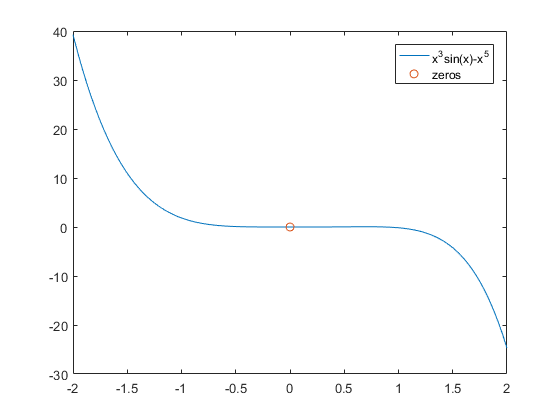
\includegraphics[width = \textwidth]{Figures/EqExample.png}
\end{figure}
A plot of the nonlinear function: $y = x^3\sin(x)-x^5$
\end{column}
\end{columns}
\end{frame}



% \begin{frame}
% \frametitle{Nominal Motion}
% \small
% \begin{columns}
% \begin{column}{0.5\textwidth}
% \textbf{Stability of a \textit{Motion}}\\
% Whether a system will remain close to its original trajectory if slightly perturbed away from it.\\
% \vspace{6pt}
% Let $\mathbf{x}^*(t)$ be the solution of the autonomous system 
% \begin{equation*}
% \dot{\mathbf{x}} = \mathbf{f(x)} \quad \& \quad \mathbf{x}^*(0) = \mathbf{x}_0
% \end{equation*}
% \vspace{6pt}
% If we perturb the initial condition to\\
% $\mathbf{x}(0) = \mathbf{x}_0 + \delta \mathbf{x}_0$ and study the associated variation of the motion error $\mathbf{e}(t) = \mathbf{x}(t) - \mathbf{x}^*(t)$
% \begin{eqnarray*}
% \mathbf{\dot{x}}^*=\mathbf{f(x^*)}  & \& & \mathbf{x}(0) = \mathbf{x}_0\\
% \mathbf{\dot{x}}=\mathbf{f(x)}  & \& &  \mathbf{x}(0) = \mathbf{x}_0 + \mathbf{\delta x}_0
% \end{eqnarray*}

% \end{column}
% \begin{column}{0.5\textwidth}
% \small
% \begin{center}
% 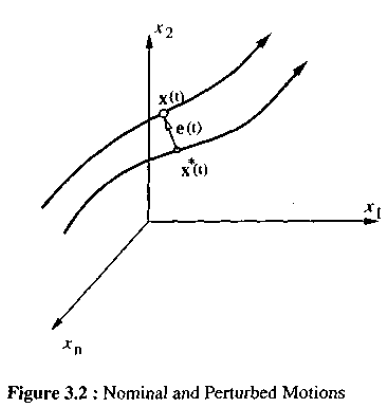
\includegraphics[width = 0.5\textwidth]{Figures/Fig32.PNG}
% \end{center}
% We have dynamics:
% \begin{eqnarray*}
% \mathbf{\dot{e}} &=& \mathbf{f}(\mathbf{x},t) - \mathbf{f}(\mathbf{x^*},t)\\
% &=& \mathbf{f}(\mathbf{x}^* + \mathbf{e},t) - \mathbf{f}(\mathbf{x^*},t)=\mathbf{g}(\mathbf{e},t)
% \end{eqnarray*}
% With initial condition: $\mathbf{e}(0) = \delta \mathbf{x}_0$. Since $\mathbf{g}(\mathbf{0},t) = \mathbf{0}$ it has equilibrium  at $\mathbf{0}$. More importantly the error is non-autonomous which we go into more detail later. 
% \end{column}
% \end{columns}
% \end{frame}

% \begin{frame}
% \frametitle{Nominal Motion Example}
% \small
% \textbf{Spring-Mass-Damper System:}\\
% Give the dynamics:
% \begin{equation*}
% m\ddot{x} + k_1 x + k_2 x^3 = 0
% \end{equation*}
% If we slightly perturb the initial position to be $x(0) = x_0 + \delta x_0$ The resulting trajectory is $x(t)$. Then the differential equation governing the motion error $e$ obeys the dynamics:
% \begin{equation*}
% m\ddot{e} + k_1 e + k_2 [e^3 + 3e^2x^*(t) + 3ex^{*2}(t)] = 0
% \end{equation*}
% Since this is a non-autonomous system, we will have to investigate more ways of solving this later.
% \end{frame}

\begin{frame}
\frametitle{Concepts of Stability}
Let $\mathbf{B}_R$ denote the spherical region (or ball) defined by $|| \mathbf{x}||<R$ in state-space.\\
\vspace{6pt}
Let $\mathbf{S}_R$ be the sphere itself, defined by $|| \mathbf{x} || = R$.\\
\vspace{6pt}
\textbf{Stable and Unstable}\\
The equilibrium state $\mathbf{x}= \mathbf{0}$ is said to be \underline{stable} if, for any $R>0$, there exists $r>0$, such that if $||\mathbf{x}(0)||<r$, then $||\mathbf{x}(t)||<R$ for all $t \geq 0$. Otherwise the equilibrium point is \underline{unstable}.
\end{frame}

\begin{frame}
\frametitle{Concepts of Stability}
\small
\begin{columns}
\begin{column}{0.5\textwidth}
\textbf{Stable}\\
Given that we do not want the state trajectory $\mathbf{x}(t)$ to get out of a ball $\mathbf{B}_R$, a starting state from within a ball $\mathbf{B}_r$ at a time 0 guarantees that the state will stay within the ball $\mathbf{B}_R$ thereafter.\\
\vspace{6pt}
\textbf{Unstable}\\
If there exists at least one ball $\mathbf{B}_R$, such that for every $r>0$ no matter how small, it is always possible for the system trajectory to start somewhere within the ball $\mathbf{B}_r$ and eventually leave the ball $\mathbf{B}_R$
\end{column}
\begin{column}{0.5\textwidth}
\begin{figure}
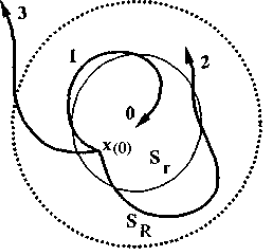
\includegraphics[width = 0.8\textwidth]{Figures/Fig33.PNG}
\end{figure}
\begin{enumerate}
\item Asymptotically Stable
\item Marginally Stable
\item Unstable
\end{enumerate}
\end{column}
\end{columns}
\end{frame}

\begin{frame}
\frametitle{Asymptotic Stability and Exponential Stability}
\small
An equilibrium point $\mathbf{0}$ is \underline{asymptotically stable} if it is stable, and if in addition there exists some $r>0$ such that $||\mathbf{x}(0)||<r$ implies that $\mathbf{x}(t) \rightarrow \mathbf{0}$ as $t \rightarrow \infty$.\\
\vspace{6pt}
An equilibrium point which is \textit{Lyapunov Stable} but not asymptotically stable is called \underline{marginally stable}. (i.e. a stability which does not necessarily approach $\mathbf{0}$ as $t \rightarrow \infty$, but stays within a ball $\mathbf{B}_R$.\\
\vspace{6pt}
An equilibrium point $\mathbf{0}$ is \underline{exponentially stable} if there exists two strictly positive numbers $\alpha$ and $\lambda$ s.t.
\begin{equation*}
\forall \; t > 0 \; , \; ||\mathbf{x}(t)|| \leq \alpha ||\mathbf{x}(0)|| e^{-\lambda t}
\end{equation*}
in some ball $\mathbf{B}_r$ around the origin.\\
\vspace{6pt}
Exponential Stability $\Rightarrow$ Asymptotic Stability $\Rightarrow$ Lyapunov Stability\\
\vspace{6pt}
If asymptotic (or exponential) stability holds for any initial states, the equilibrium point is said to be asymptotically (or exponentially) stable \underline{in the large}. It is also called \underline{globally} asymptoticly (or exponentially) stable. 
\end{frame}

\begin{frame}
\frametitle{Linearization and Local Stability}
\small
\textbf{Linearization}\\
Lyapunov's linearization method is concerned with the local stability of a nonlinear system. Concerning $\mathbf{f(x)} \in C^1$ (Cont. differentiable at least once). The dynamics may be Taylor Series approximated about the equilibrium $\mathbf{x = 0}$:
\begin{equation*}
\mathbf{\dot{x}} = \left. \left( \frac{\partial \mathbf{f}}{\partial \mathbf{x}} \right) \right. _{\mathbf{x = 0}}\mathbf{x} + \mathbf{f}_{h.o.t.}(\mathbf{x})
\end{equation*}
If we define the Jacobian as $\mathbf{A}$, we have the linear system:
\begin{equation*}
\mathbf{\dot{x} = Ax}
\end{equation*}
Consider a nonlinear non-autonomous nonlinear system with control $\mathbf{u}$: 
\begin{equation*}
\mathbf{\dot{x} = \left. \left( \frac{\partial \mathbf{f}}{\partial \mathbf{x}} \right) \right. _{\mathbf{x=0,u = 0}}\mathbf{x} + \left. \left( \frac{\partial \mathbf{f}}{\partial \mathbf{u}} \right) \right. _{\mathbf{x=0,u = 0}}\mathbf{u} + \mathbf{f}_{h.o.t.}}
\end{equation*}
Defining the Jacobians:
\begin{equation*}
\mathbf{\dot{x}=Ax+Bu}
\end{equation*}
\end{frame}

\begin{frame}
\frametitle{Linearization and Local Stability}
\Large
\textbf{Lyapunov's Linearization Method}\\
\small
\begin{itemize}
\item \textbf{Asymptotically Stable} All $\text{eig}(\mathbf{A}) < 0$\\
\vspace{6pt}
If the linearized system is strictly stable (all eigenvalues of $\mathbf{A}$ are strictly in the L.H.P.) then the equilibrium point is asymptotically stable (for the actual nonlinear system)\\
\vspace{3pt}
\item \textbf{Unstable} At least one $\text{eig}(\mathbf{A}) > 0$\\
\vspace{6pt}
If the linearized system is unstable (i.e. if at least one eigenvalue of $\mathbf{A}$ is strictly in the R.H.P.), then the equilibrium point is unstable (for the nonlinear system).\\
\vspace{3pt}
\item \textbf{Indeterminate} At least one eigenvalue is on the $j\omega$ axis.\\
\vspace{6pt}
If the linearized system is marginally stable (i.e. all eigenvalues of $\mathbf{A}$ are in the left-hand complex plane, but at least one of them is on the $j\omega$ axis), then on cannot conclude anything form the linear approximation (the equilibrium point may be stable, asymptoticly stable, or unstable for the nonlinear system).
\end{itemize}
\end{frame}

\begin{frame}
\frametitle{Linearization and Stability Example}
\small
\textbf{Given:}\\
Let $x_1 = x$ and $x_2 = \dot{x}$. The state space representation is:
\begin{equation*}
\begin{aligned}
\dot{x}_1 &= x_2 = f_1(\mathbf{x})\\
\dot{x}_2 &= x_1^3sin^3(x_1) - x_1^5 - (x_1-1)^4x_2^7 = f_2(\mathbf{x})
\end{aligned}
\end{equation*}
Determine the stability of the equilibrium point at the origin determined earlier.
\begin{equation*}
\mathbf{A} = \frac{\partial \mathbf{f}}{\partial \mathbf{x}} = \begin{bmatrix}
\frac{\partial f_1}{\partial x_1} & \frac{\partial f_1}{\partial x_2} \\
\frac{\partial f_2}{\partial x_1} & \frac{\partial f_2}{\partial x_2}
\end{bmatrix}
\end{equation*}
Computing:
\begin{equation*}
\begin{aligned}
\frac{\partial f_1}{\partial x_1} &= 0 \;\; \& \;\; \frac{\partial f_1}{\partial x_2} = 1\\
\frac{\partial f_2}{\partial x_1} &= 3 x_1^2 \sin^3(x_1) - 4 x_2^7 (x_1 - 1)^3 - 5 x_1^4 + 3 x_1^3 \cos(x_1) \sin(x_1)^2
\\
\frac{\partial f_2}{\partial x_2} &= -7 x_2^6 (x_1 - 1)^4
\end{aligned}
\end{equation*}
\end{frame}

\begin{frame}
\frametitle{Linearization and Stability Example}
\small
Recall the Linearization was:
\begin{equation*}
\tiny
\mathbf{A} = \begin{bmatrix}
0 & 1\\
3 x_1^2 \sin^3(x_1) - 4 x_2^7 (x_1 - 1)^3 - 5 x_1^4 + 3 x_1^3 \cos(x_1) \sin(x_1)^2 & -7 x_2^6 (x_1 - 1)^4
\end{bmatrix}
\end{equation*}
If we evaluate the linearization:
\begin{equation*}
\left. \mathbf{A}\right.|_{\mathbf{x}_eq} = \begin{bmatrix}
0 & 1\\ 0&0
\end{bmatrix}
\end{equation*}
Finding the eigenvalues of $\mathbf{A}$, \texttt{eig}$(\mathbf{A}) = [0,0]$.
We can not conclude the stability of the origin using the linearization method. Instead we will need to introduce a more rigorous method if we would like to ascertain the stability of the origin for our toy problem.
\end{frame}


\begin{frame}
\frametitle{Lyapunov's Direct Method}
\small
\textbf{Idea:} If the total energy of a mechanical (or electrical system) is continuously dissipated, then the system, whether linear or nonlinear, must eventually settle down to an equilibrium point.\\
\vspace{6pt}
\begin{columns}
\begin{column}{0.5\textwidth}
The Total Energy of the System:
\begin{eqnarray*}
V(x) &=& \frac{1}{2} m \dot{x}^2 + \int_0^x (k_0 x + k_1 x^3) dx\\
&=& \frac{1}{2}m\dot{x}^2 + \frac{1}{2}k_0 x^2 + \frac{1}{4} k_1 x^4
\end{eqnarray*}
- Zero energy corresponds to the equilibrium point ($x = 0, \dot{x} = 0$)\\
- Asymptotic stability implies the convergence of mechanical energy to zero\\
- Instability is related to the growth of mechanical energy\\
\end{column}
\begin{column}{0.5\textwidth}
\begin{center}
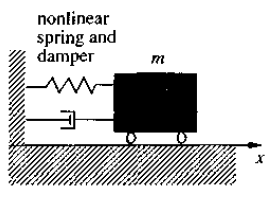
\includegraphics[width = 0.4\textwidth]{Figures/Fig36.PNG}
\end{center}
Rate of Energy Variation:
\begin{eqnarray*}
\dot{V}(x) &=& m \dot{x} \ddot{x} + (k_0 x + k_1 x^3)\dot{x}\\
&=& \dot{x}(-b\dot{x}|\dot{x}|)\\
&=& -b |\dot{x}|^3
\end{eqnarray*}
 The energy of the system, starting from some initial value, is continuously dissipated by the damper until the mass settles down. ($\dot{x}=0$.)
\end{column}
\end{columns}
\end{frame}

\begin{frame}
\frametitle{Positive Definite Functions and Lyapunov Functions}
The energy function has two properties:
\begin{itemize}
\item The Lyapunov functions is strictly positive unless both state variables $x$ and $\dot{x}$ are zero.
\item the function is monotonically decreasing when the variables $x$ and $\dot{x}$ vary according to the dynamics.
\end{itemize}
A scalar continuous function V(x) is said to be \underline{locally positive definite} if $V(0) = 0$ and, in a ball $B_{R_0}$, $\mathbf{x} \neq \mathbf{0} \Rightarrow V(\mathbf{x})>0$\\
\vspace{6pt}
If $V(\mathbf{0})=0$ and the above property holds over the whole state space, then $V(\mathbf{x})$ is said to be \underline{globally positive definite}.\\
For instance, the function of the mechanical energy of a pendulum:\\
\begin{equation*}
V(\mathbf{x}) = \frac{1}{2}MR^2 x_2^2 + MRg(1-\cos x_1)
\end{equation*}
\end{frame}

\begin{frame}
\frametitle{Positive Definite Functions and Lyapunov Functions}
\begin{columns}
\begin{column}{0.5\textwidth}
\textbf{Shape of Positive Definite Function}\\
Describing the geometrical meaning of locally positive definite functions. Consider a positive definite function $V(\mathbf{x})$ of two state variables $x_1$ and $x_2$. Plotted in 3-D, $V(\mathbf{x})$ typically corresponds to a surface looking like an upward cup. The lowest point of the cup is located at the origin.
\end{column}
\begin{column}{0.5\textwidth}
\begin{center}
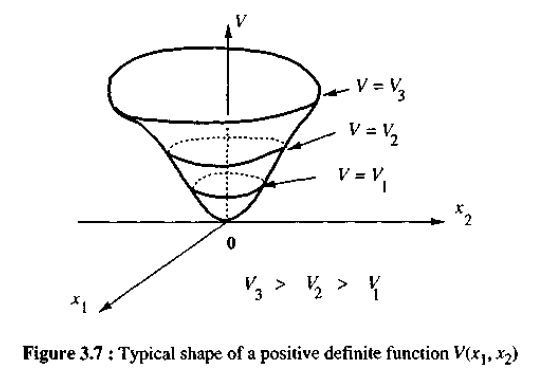
\includegraphics[width = \textwidth]{Figures/Fig37.PNG}
\end{center}
\end{column}
\end{columns}
\end{frame}

\begin{frame}
\frametitle{Positive Definite Functions and Lyapunov Functions}
\begin{columns}
\begin{column}{0.5\textwidth}
\textbf{Level Curves}\\
A second geometrical representation can be made by taking $x_1$ and $x_2$ as Cartesian coordinates. The level curves $V(x_1,x_2) = V_\alpha$ represent a set of curves corresponding to an energy level. Think of this as a topology graph where each band is a level of energy rather than altitude.
\end{column}
\begin{column}{0.5\textwidth}
\begin{center}
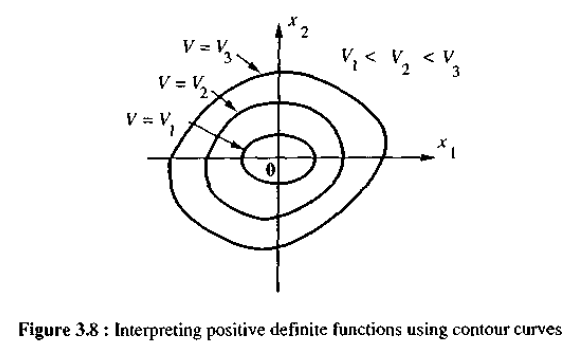
\includegraphics[width = \textwidth]{Figures/Fig38.PNG}
\end{center}
\end{column}
\end{columns}
\end{frame}

\begin{frame}
\frametitle{Positive Definite Functions and Lyapunov Functions}
\small
\begin{columns}
\begin{column}{0.5\textwidth}
A few related concepts can be defined for a local or global sense\\
\vspace{6pt}
\begin{itemize}
\item A function $V(\mathbf{x)}$ is \underline{negative definite} if $-V(\mathbf{x})$ is positive definite.
\item A function $V(\mathbf{x})$ is \underline{semi-definite} if $V(\mathbf{0}) = 0$ and $V(\mathbf{x}) \geq \mathbf{0} \; \forall \; \mathbf{x} \neq \mathbf{0}$.
\item $V(\mathbf{x})$ is \underline{negative semi-definite} if $-V(\mathbf{x})$ is positive semi-definite
\end{itemize}
\vspace{0.6pt}
Assuming that the scalar function $V(\mathbf{x})$ is implicit in time, we can find its time derivative by the chain rule:
\begin{equation*}
\dot{V} = \frac{d V(\mathbf{x})}{d t} = \frac{\partial V}{\partial \mathbf{x}} \mathbf{\dot{x}} = \frac{\partial V}{\partial \mathbf{x}} \mathbf{f(x)}
\end{equation*}
\end{column}
\begin{column}{0.5\textwidth}
If, in a ball $\mathbf{B}_{R_0}$, the function $V(\mathbf{x})$ is \textit{positive definite} and has continuous partial derivatives, and if its time derivative along any state trajectory of $\mathbf{\dot{x} = f(x)}$ is \textit{negative semi-definite}:
\begin{equation*}
\dot{V(}\mathbf{x}) \leq 0
\end{equation*}
then $V(\mathbf{x})$ is said to be a \underline{Lyapunov Function} for the system: $\mathbf{\dot{x} = f(x)}$.
\begin{center}
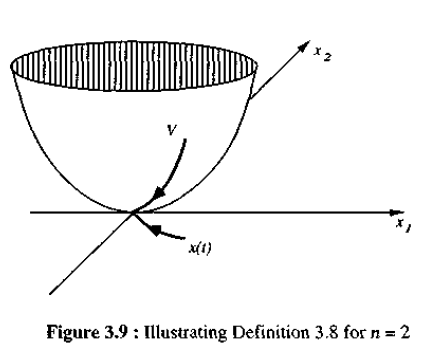
\includegraphics[width = 0.7\textwidth]{Figures/Fig39.PNG}
\end{center}
\end{column}
\end{columns}
\end{frame}

\begin{frame}
\frametitle{Equilibrium Point Theorems}
\small
\begin{columns}
\begin{column}{0.5\textwidth}
\textbf{Thm 3.2 Local Stability:}\\
If, in a ball $\mathbf{B}_{R_0}$ there exists a scalar function $V(\mathbf{x})$ with continuous first partial derivatives such that:
\begin{itemize}
\item $V(\mathbf{x})$ is positive definite (locally in $\mathbf{B}_{R_0}$)
\item $\dot{V}(\mathbf{x})$ is negative semi-definite (locally in $\mathbf{B}_{R_0}$)
\end{itemize}
Then the equilibrium point $\mathbf{0}$ is stable. \\ \vspace{6pt}
If actually, the derivative $\dot{V}(\mathbf{x})$ is locally \textit{negative definite} in $\mathbf{B}_{R_0}$, then the stability is asymptotic.\\
\vspace{6pt}
\textit{Proof in Slotine and Li pp. 62}
\end{column}
\begin{column}{0.5\textwidth}
\textbf{Example: Pendulum Local Stability}\\
Consider: $\ddot{\theta} + \dot{\theta} + \sin(\theta) = 0$ and the scalar function describing the sum of potential and kinetic energy:
\begin{equation*}
V(\mathbf{x}) = (1-\cos\theta)+\dot{\theta}^2/2
\end{equation*}
with time derivative:
\begin{equation*}
\dot{V(\mathbf{x})} = \dot{\theta} \sin \theta + \dot{\theta} \ddot{\theta} = - \dot{\theta}^2 \leq 0
\end{equation*}
The origin is a locally stable equilibrium point. Since $V(\mathbf{x}) \leq 0$ we can not conclude if stability is asymptotic.
\end{column}
\end{columns}
\end{frame}

\begin{frame}
\frametitle{Positive Definite Functions and Lyapunov Functions}
\small
\textbf{Example: Asymptotic Stability}\\
Consider:\\
\begin{equation*}
\begin{aligned}
\dot{x}_1 &= x_1 (x_1^2 + x_2^2 - 2) - 4x_1x_2^2\\
\dot{x}_2 &= 4x_1^2x_2 + x_2(x_1^2 + x_2^2 - 2)
\end{aligned}
\end{equation*}
Given the Positive Definite Function:
\begin{equation*}
V(\mathbf{x}) = x_1^2 + x_2^2
\end{equation*}
and its time derivative:
\begin{equation*}
\dot{V}(\mathbf{x}) = 2(x_1^2 + x_2^2)(x_1^2 + x_2^2 - 2)
\end{equation*}
About the origin, $\dot{V}$ is negative definite and the Thm. dictates that the origin is asymptotically stable.
\end{frame}


\begin{frame}
\frametitle{Lyapunov Theorem for Global Stability}
\small 
\begin{columns}
\begin{column}{0.5\textwidth}
\textbf{Theorem: (Global Stability)}\\
Assume that there exists a scalar function $V$ of the sates $\mathbf{x}$ with continuous first order derivatives such that:
\begin{itemize}
\item $V(\mathbf{x})$ is positive definite
\item $\dot{V}(\mathbf{x})$ is negative definite
\item $V(\mathbf{x}) \rightarrow \infty$ as $||\mathbf{x}|| \rightarrow \infty$
\end{itemize}
then the equilibrium at the origin is \underline{globally asymptotically stable}.\\
\vspace{6pt}
The reason for the radial unboundedness condition is to assure that the contour curves correspond to closed curves. 
\end{column}
\begin{column}{0.5\textwidth}
If the curves are not closed state trajectories could drift away from the equilibrium point if the state keeps going through contours corresponding to lower $V_\alpha$.\\
Consider: $V(\mathbf{x}) = \frac{x_1^2}{1+x_1^2} + x_2^2$\\
The Curves $V(\mathbf{x}) = V_\alpha$ for $V_\alpha > 1$ are open curves, demonstrating divergence the state while moving toward lower ``energy.''
\begin{center}
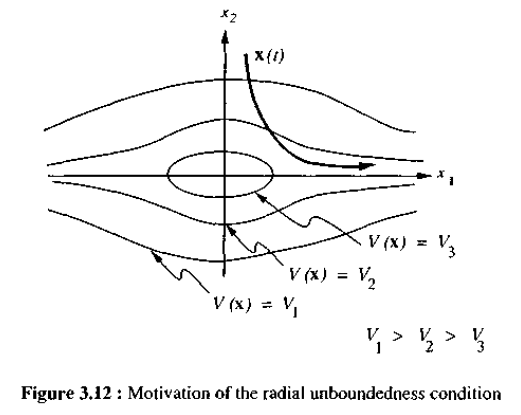
\includegraphics[width = 0.8\textwidth]{Figures/Fig312.PNG}
\end{center}
\end{column}
\end{columns}
\end{frame}

\begin{frame}
\frametitle{Lyapunov Theorem for Global Stability}
\textbf{A Class of First Order Systems Example:}\\
Consider: $\dot{x} + c(x) = 0$, where $c$ is any continuous function of the same sign as its scalar argument $x$. (\textit{odd function}).\\
\vspace{6pt}
Consider the Lyapunov Function and its derivative:
\begin{equation*}
V = x^2 \;\; \& \;\; \dot{V} = 2 x \dot{x} = -2xc(x)
\end{equation*}
The function $V$ is radially unbounded since it tends towards infinity as $|x| \rightarrow \infty$. And the Derivative is negative definite as long as $x \neq 0$.\\
\vspace{6pt}
Therefore: the origin $x=0$ is \textit{Globally Asymptotically Stable} equilibrium point.\\
Note that the global nature implies that the origin is the only equilibrium point.
\end{frame}

\begin{frame}
\frametitle{Systems Analysis Based Upon Lyapunov's Direct  Method}
\textbf{Question:} How do we find a Lyapunov function for a specific probelem?\\
\textbf{Answer:} There is \underline{no general way} of finding Lyapunov functions for nonlinear systems. \textit{Experience, Intuition, and Physical Insight} are required to search for candidate Lyapunov functions.\\
\vspace{6pt}
\textbf{Methods to Assist with Finding Lyapunov Functions}
\begin{itemize}
\item Lyapunov Analysis of LTI Systems
\item Krasovskii's Method
\item Variable Gradient Method
\end{itemize}
\end{frame}

\begin{frame}
\frametitle{Matrix Mathematics Reminder}
\small
\textbf{Square Symmetric Matrix}\\
A square matrix is \underline{symmetric} iff a square matrix $M$ satisfies the following:\\
\begin{equation*}
\mathbf{M} = \mathbf{M^T}
\end{equation*}
\textbf{Square Skew Symmetric Matrix}\\
A square matrix is \underline{skew-symmetric} iff a square matrix $M$ satisfies the following:\\
\begin{equation*}
\mathbf{M} = -\mathbf{M^T}
\end{equation*}
\textbf{Composition of a Square Matrix}\\
Any square matrix, $\mathbf{M}$ may be composed into its symmetric and skew-symmetric parts:
\begin{equation*}
\mathbf{M} = \frac{\mathbf{M}+\mathbf{M^T}}{2} + \frac{\mathbf{M} - \mathbf{M^T}}{2}
\end{equation*}
\end{frame}

\begin{frame}
\frametitle{Matrix Mathematics Reminder}
\small
\textbf{Necessary and Sufficient Criteria for Skew-Symmetric Matrix}\\
The quadratic function associated with a skew-symmetric matrix is always zero. If $\mathbf{M}$ is a square skew-symmetric matrix then:
\begin{equation*}
\mathbf{x^TMx} = \mathbf{-x^TMx} = \mathbf{0} \; \forall \; \mathbf{x} \in \mathbb{R}^n , \mathbf{M} \in \mathbb{R}^{n \times n}
\end{equation*}
\vspace{6pt}

\textbf{Positive Definite Matrix}\\
A square matrix $\mathbf{M}$ is positive definite if
\begin{equation*}
\lbrace \mathbf{x^TMx} > 0 | \; \forall \; \mathbf{x \neq 0} \in \mathbb{R}^n , \mathbf{M} \in \mathbb{R}^{n \times n} \rbrace
\end{equation*}\\
We can also say a necessary condition is that all the minors of $\mathbf{M}$ are strictly positive.
\vspace{6pt}
\end{frame}

\begin{frame}
\frametitle{Lyapunov Analysis of LTI Systems}
\small
Given a Linear Time-Invariant System:
\begin{equation*}
\mathbf{\dot{x} = Ax} \; | \; \mathbf{x}\in\mathbb{R}^n , \mathbf{A}\in\mathbb{R}^{n\times n}
\end{equation*}
Consider the quadratic Lyapunov function candidate, with $\mathbf{P}$ symmetric and positive definite:
\begin{equation*}
\mathbf{V = x^T P x} \; | \; \mathbf{P} = \mathbf{P}^T , \mathbf{P>0}
\end{equation*}
Taking the time derivative:
\begin{equation*}
\begin{aligned}
\mathbf{\dot{V}} &= \mathbf{\dot{x}^T P x + x^T\dot{P}x + x^T P\dot{x}}\\
&= \mathbf{\dot{x}^T P x + x^T P\dot{x}}\\
&= \mathbf{(x^T A^T) P x + x^T P (A x)}\\
&= \mathbf{x^T (A^T P +  P A) x}\\
&= -\mathbf{x^T Q x}
\end{aligned}
\end{equation*}
$\mathbf{Q} >0 \Rightarrow$  the origin is Globally Asymptotically Stable (GAS).
\end{frame}

\begin{frame}
\frametitle{Example Lyapunov Analysis of LTI Systems}
\small
Given a Linear Time-Invariant System:
\begin{equation*}
\mathbf{\dot{x} = \begin{bmatrix}
0 & 4 \\ -8 & -12
\end{bmatrix}x}
\end{equation*}
Let us choose a positive definite $\mathbf{Q}$, then solve for the $\mathbf{P}$ using:
\begin{equation*}
\mathbf{A^T P + P A = -Q}
\end{equation*}
satisfying the quadratic form we then determine if $\mathbf{P}>0$:
\begin{equation*} 
\begin{bmatrix}
p_{11} & p_{12}\\p_{21} & p_{22}
\end{bmatrix} 
\begin{bmatrix}
0 & 4 \\ -8 & -12
\end{bmatrix}
+
\begin{bmatrix}
0 & -8 \\ 4 & -12
\end{bmatrix}
\begin{bmatrix}
p_{11} & p_{12}\\p_{21} & p_{22}
\end{bmatrix}  = 
\begin{bmatrix}
-1 & 0 \\ 0 & -1\end{bmatrix} 
\end{equation*}
\begin{equation*}
\begin{aligned}
-8 p_{12} - 8 p_{21} &= -1\\
4 p_{11} -12 p_{12} - 8 p_{22} &= 0\\
-8 p_{22} + 4 p_{11} -12 p_{21} & = 0\\
4 p_{21} -12 p_{22} + 4 p_{12} -12 p_{22} &= -1
\end{aligned}
\end{equation*}
Solving 
\begin{equation*}
\mathbf{P} = \begin{bmatrix}
5/16 & 1/16 \\
1/16 & 1/16
\end{bmatrix}
\end{equation*}
$\mathbf{P} >0 \therefore$  the origin is Globally Asymptotically Stable (GAS).
\end{frame}

\begin{frame}
\frametitle{Krasovskii's Method}
\small
\textbf{Consider:} $\mathbf{\dot{x} = f(x)}$ with equilibrium at the origin.\\
\vspace{6pt}
We are going to choose a quadratic function $V = \mathbf{f^T(x) f(x)}$ and check whether this particular choice leads to a \underline
{Lyapunov function}\\
\vspace{6pt}
Taking the time derivative of the Lyapunov Function Candidate:
\begin{equation*}
\begin{aligned}
\dot{V}(\mathbf{x}) = \mathbf{\dot{f}^T(x)f(x)} + \mathbf{f^T(x)\dot{f}(x)}
\end{aligned}
\end{equation*}
If we define $\mathbf{A} = \frac{\partial f}{\partial x}$ be the Jacobian, then:
\begin{equation*}
\begin{aligned}
\dot{V}(\mathbf{x}) &= \frac{\partial f}{\partial x} \frac{dx}{dt} = \mathbf{A}(\mathbf{x})\dot{\mathbf{x}}\\
&= \mathbf{f^T(x)(A+A^T)f(x)}
\end{aligned}
\end{equation*}
If the matrix $\mathbf{F = A+A^T}$ is negative definite in the neighborhood $\mathbf{\Omega}$ then the equilibrium point at the origin is \underline{asymptotically stable}.\\
\vspace{6pt}
Further if $\mathbf{F}<0$ and $||\mathbf{x}|| \rightarrow \infty
$ as $V(\mathbf{x}) \rightarrow \infty$, then the equilibrium is \underline{Globally Asymptotically Stable}.
\end{frame}

\begin{frame}
\frametitle{Krasovskii's Method}
\small
\textbf{Downsides:}
\begin{itemize}
\item $\mathbf{F}$ may not be negative definite
\item For higher order systems, tough to check $\mathbf{F} < 0 \; \forall \; \mathbf{x}$
\end{itemize}
\textbf{Example:}
\begin{equation*}
\begin{aligned}
\dot{x}_1 &= -6 x_1 + 2x_2\\
\dot{x}_2 &= 2 x_1  - 6x_2 - 2x_2^3
\end{aligned}
\end{equation*}
From this:
\begin{equation*}
\mathbf{A(x)} = \frac{\partial \mathbf{f}}{\partial \mathbf{x}} = \begin{bmatrix}
-6 & 2\\2 & -6 - 6x_2^2
\end{bmatrix} \quad \& \quad \mathbf{F = A+ A^T} = \begin{bmatrix}
-12 & 4\\4 & -12 -12 x_2^2
\end{bmatrix}
\end{equation*}
Looking at the determinate, it is easy to show that the function $\mathbf{F}$ is \underline{negative definite} for all $\mathbf{x}$. \\
\vspace{6pt}
The Lyapunov Function is: 
\begin{equation*}
\begin{aligned}
V(\mathbf{x}) &= 
\begin{bmatrix}
-6 x_1 + 2x_2 &
2 x_1 - 6x_2 - 2x_2^3
\end{bmatrix}
\begin{bmatrix}
-6 x_1 + 2x_2 \\
2 x_1 - 6x_2 - 2x_2^3
\end{bmatrix}\\
 &= (-6 x_1 + 2x_2)^2 + (2 x_1 - 6 x_2 - 2x_2^3)^2
\end{aligned}
\end{equation*}
Since $V \rightarrow \infty$ as $||\mathbf{x}|| \rightarrow \infty$ the origin is GAS.
\end{frame}

\begin{frame}
\frametitle{Variable Gradient Method}
\small
The \underline{Variable Gradient Method} is a \textit{Formal Approach} to construction Lyapunov functions. In involves assuming a form for the gradient of an unknown Lyapunov function, and then finding the Lyapunov function itself by integrating the assumed gradient.\\
\vspace{6pt}
For a Scalar Function:
\begin{equation*}
\dot{\mathbf{x}} = \lbrace \left. f(\mathbf{x}) \Rightarrow x_i = f_i(\mathbf{x}) \;  | \; i = \lbrace 1,2,\; ... \;, n \rbrace \right. \rbrace
\end{equation*}
Given, $V(\mathbf{x}) \in C^1$ (continuously differentiable at least once) then:
\begin{equation*}
\dot{V}(\mathbf{x}) = \left[ \frac{\partial V}{\partial \mathbf{x}}\right] \dot{\mathbf{x}} = \sum_i  \frac{\partial V}{\partial x_i} \dot{x}_i = \sum_i \frac{\partial V}{\partial x_i} f_i(\mathbf{x}) = g\mathbf{^T}(\mathbf{x})\mathbf{f(x)}
\end{equation*}
Where: $g(\mathbf{x}) = \nabla V(\mathbf{x})$.
\end{frame}

\begin{frame}
\frametitle{Variable Gradient Method}
\small
Remember, we get to pick $g(\mathbf{x})$ to get a unique scalar function $V(\mathbf{x})$.\\
\vspace{6pt}
Using the Vector Gradient Method, $V(\mathbf{x})$ must satisfy the \textbf{Curl Conditions}:
\begin{equation*}
\frac{\partial \nabla V_i}{\partial x_j} = \frac{\partial \nabla V_j}{\partial x_i} \quad , (i,j = 1,2,...,n)
\end{equation*}
or in terms of $g(\mathbf{x})$
\begin{equation*}
\frac{g_i(\mathbf{x)}}{\partial x_j} = \frac{\partial g_j (\mathbf{x})}{\partial x_i} \quad , (i,j = 1,2,...,n)
\end{equation*}
The \textbf{Curl Conditions} imply that the integration of $\dot{V}$ to $V$ will be independent of integration path. The integration is as follows:
\begin{equation*}
\begin{split}
V(\mathbf{x}) =& \int_0^{x_1} g_1(\chi_1,0,...,0) d\chi_1 +  \int_0^{x_2} g_2(\chi_1,\chi_2,...,0) d\chi_2 + \\  & \quad \int_0^{x_n} g_n(\chi_1,\chi_2,...,\chi_n) d\chi_n
\end{split}
\end{equation*}
So all we need is  $g(\mathbf{x})$, the gradient. Let's select $g_i(\mathbf{x}) = \sum_{j = 1}^{n} a_{ij} x_j$ where $a_{ij}$ are selected to satisfy the curl conditions.
\end{frame}

\begin{frame}
\frametitle{Vector Gradient Method}
\small
\textbf{Example:}
\begin{equation*}
\begin{aligned}
\dot{x}_1 &= -2 x_1\\
\dot{x}_2 &= -2 x_2 + 2x_1 x_2 ^2
\end{aligned}
\end{equation*}
Selecting the gradient function $g_i(\mathbf{x}) = \sum_{j = 1}^{n} a_{ij} x_j$ where $a_{ij}$ are selected to satisfy the curl
\begin{equation*}
\begin{aligned}
g_1(\mathbf{x}) &= a_{11} x_1 + a_{12} x_2\\
g_2(\mathbf{x}) &= a_{21} x_1 + a_{22} x_2
\end{aligned}
\end{equation*}
Satisfying the Curl Conditions:
\begin{equation*}
\frac{\partial g_1}{\partial x_2} = \frac{\partial g_2}{\partial x_1} \Rightarrow a_{12} + x_2 \frac{\partial a_{12}}{\partial x_2} = a_{21} +  x_1 \frac{\partial a_{21}}{\partial x_1} 
\end{equation*}
If we select $a_{12} = a_{21} = 0$ and let $a_{11} = a_{22} = 1$, then:
\begin{equation*}
\begin{aligned}
g_1(\mathbf{x}) &= x_1\\
g_2(\mathbf{x}) &= x_2
\end{aligned}
\end{equation*}
Now: $\dot{V}(\mathbf{x}) = \mathbf{g^T f} = \begin{bmatrix}
x_1 & x_2
\end{bmatrix}
\begin{bmatrix}
-2 x_1 \\ -2 x_2 + 2 x_1 x_2^2
\end{bmatrix} = -2x_1^2 - 2x_2^2 (1-x_1x_2)$
\end{frame}


\begin{frame}
\frametitle{Vector Gradient Method}
\small
\textbf{Example Cont.}
\begin{equation*}
\dot{V}(\mathbf{x}) = \mathbf{g^T f} = \begin{bmatrix}
x_1 & x_2
\end{bmatrix}
\begin{bmatrix}
-2 x_1 \\ -2 x_2 + 2 x_1 x_2^2
\end{bmatrix} = -2x_1^2 - 2x_2^2 (1-x_1x_2)
\end{equation*}
So for \underline{Negative Definite} $\dot{V}$ we need $(1-x_1 x_2)>0$ As long as we stay in this domain, then $\dot{V}$ will be negative definite.\\
\vspace{6pt}
Integrating:
\begin{equation*}
V(\mathbf{x}) = \int_0^{x_1} \chi_1 d\chi_1 + \int_0^{x_2} \chi_2 d\chi_2 = \frac{1}{2}(x_1^2 + x_2^2)
\end{equation*}
This is obviously P.D. and therefore this system is \underline{Locally Asymptotically Stable} in the Domain: $(1-x_1x_2)>0$\\
\vspace{6pt}
\textbf{Example With Functions for $a_{ij}$}
Recall that we saw that $a_{ij}$ took values of constants, but what if they were function of the states?\\
\end{frame}

\begin{frame}
\frametitle{Vector Gradient Method}
\small
\textbf{Example:}
\begin{equation*}
\begin{aligned}
\dot{x}_1 &= -2 x_1\\
\dot{x}_2 &= -2 x_2 + 2x_1 x_2 ^2
\end{aligned}
\end{equation*}
Selecting the gradient function $g_i(\mathbf{x}) = \sum_{j = 1}^{n} a_{ij} x_j$ where $a_{ij}$ are selected to satisfy the curl
\begin{equation*}
\begin{aligned}
g_1(\mathbf{x}) &= a_{11} x_1 + a_{12} x_2\\
g_2(\mathbf{x}) &= a_{21} x_1 + a_{22} x_2
\end{aligned}
\end{equation*}
Satisfying the Curl Conditions:
\begin{equation*}
\frac{\partial g_1}{\partial x_2} = \frac{\partial g_2}{\partial x_1} \Rightarrow a_{12} + x_2 \frac{\partial a_{12}}{\partial x_2} = a_{21} +  x_1 \frac{\partial a_{21}}{\partial x_1} 
\end{equation*}
If we select $a_{11} = 1$, $a_{12} = x_2^2$,  $a_{21} = 3x_2^2$, and let $a_{22} = 3$, then the curl equations yield:
\begin{equation*}
\begin{aligned}
x_2^2 + x_2(2 x_2) = 3 x_2^2 + x_1(0) \quad \checkmark
\end{aligned}
\end{equation*}
The gradients are therefore:
\begin{equation*}
\begin{aligned}
g_1(\mathbf{x}) &= x_1 + x_2^3\\
g_2(\mathbf{x}) &= 3x_1 x_2^2 + 3x_2
\end{aligned}
\end{equation*}
\end{frame}

\begin{frame}
\frametitle{Vector Gradient Method}
The Lyapunov Function Rate:\\
\begin{equation*}
\begin{split}
\dot{V}(\mathbf{x}) &= \mathbf{g^Tf} = \begin{bmatrix}
x_1 + x_2^3 & 3 x_1x_2^2 + 3x_2
\end{bmatrix}\begin{bmatrix}
-2x_1\\ -2x_2 + 2x_1x_2^2
\end{bmatrix}\\
&= -2x_1(x_1+x_2^3) - (2x_2+2x_1x_2^2)(3x_1x_2^2 + 3x_2)\\
&= -2x_1^2 -2x_1x_2^3 - 6x_1x_2^3 - 6x_2^2 - 6x_1^2x_2^4 - 6x_1x_2^3
\end{split}
\end{equation*}
Which is Negative Definite. Integrating we may obtain the Lyapunov Function:
\begin{equation*}
V = x_1^2/2 + 3/2 x_2^2 + x_1 x_2^3
\end{equation*}
So we have an Asymptotically Stable Equilibrium at the origin.
\end{frame}

\begin{frame}
\frametitle{Vector Gradient Method}
\textbf{Procedure:}
\begin{enumerate}
\item Assume that $g(\mathbf{x})$ has a certain form with undetermined coefficients. ``Hard Part''
\item Solve for the coefficients by satisfying the curl conditions
\item Restrict coefficients so that $\dot{V}(\mathbf{x})$ is negative semi-definite (at least locally)
\item Compute $V(\mathbf{x})$ using integration equation
\item Check if $V(\mathbf{x})$ is Positive Definite
\end{enumerate}
\end{frame}

\begin{frame}
\frametitle{Example: Pendulum with Friction}
\small
\textbf{State Space:}
\begin{equation*}
\begin{aligned}
\dot{x}_1 &= x_2\\
\dot{x}_2 &= -\frac{g}{l}\sin x_1 - b x_2
\end{aligned}
\end{equation*}
\textbf{Step 1: Assume that $g(\mathbf{x})$ has a certain form with undetermined coefficients.}\\
\begin{equation*}
\begin{aligned}
g_i(\mathbf{x}) &= \sum_{j=1}^{n} a_{ij} x_j\\
g_1(\mathbf{x}) &= a_{11} x_1 + a_{12} x_2\\
g_2(\mathbf{x}) &= a_{21} x_1 + a_{22} x_2
\end{aligned}
\end{equation*}
\textbf{Step 2: Solve for the coefficients by satisfying the curl conditions}
\begin{equation*}
\begin{aligned}
\frac{\partial g_1}{\partial x_2} = \frac{\partial g_2}{\partial x_1} = a_{12} = a_{21} = \textrm{Const.}
\end{aligned}
\end{equation*}
\end{frame}

\begin{frame}
\frametitle{Example: Pendulum with Friction}
\small
\textbf{Step 3: Restrict coefficients so that $\dot{V}(\mathbf{x})$ is negative semi-definite}
\begin{equation*}
\begin{aligned}
&\dot{V}(\mathbf{x}) = \mathbf{g^T f}\\
&= a_{11} x_1 x_2 + a_{12} x_2^2 + ( a_{12} x_1 + a_{22} x_2 ) ( - \frac{g}{l} \sin x_1 - b x_2)\\
&= a_{11} x_1 x_2 + a_{12} x_2^2 - b a_{12} x_1 x_2 - b a_{22} x_2^2 - \frac{g}{l} a_{12} x_1 \sin x_1 - \frac{g}{l} a_{22} x_2 \sin x_1\\
&=(a_{11}-b a_{12}) x_1 x_2 + (a_{12}-b a_{22}) x_2^2 - a_{12} \frac{g}{l} x_1 \sin x_1 - a_{22} \frac{g}{l} x_2 \sin x_1
\end{aligned}
\end{equation*}
To keep $\dot{V}(\mathbf{x}) \leq 0$ we need to get rid of cross terms:
\begin{equation*}
\begin{aligned}
(a_{11} - b a_{12} = 0) & \quad \text{$x_1 x_2$ term disappear} \\
a_{22} = 0 & \quad \text{$x_2 \sin x_1$ term disappear}\\
a_{11} - b a_{22} < 0 & \quad  \text{Because $x_2^2$ is P.D.}
\end{aligned}
\end{equation*}
Only way is to make the coefficients all zero. Which is bad! We will need a different $g(\mathbf{x})$.
\end{frame}

\begin{frame}
\frametitle{Example Pendulum with Friction}
\small
\textbf{Step 1: Assume that $g(\mathbf{x})$ has a certain form with undetermined coefficients}. We will have to add a trig term to one or both of the $g_i(\mathbf{x})$'s. Let's try:
\begin{equation*}
\begin{aligned}
g_1(\mathbf{x}) &= a_{11}x_1 + \frac{g}{l} \sin x_1 + a_{12}x_2\\
g_2(\mathbf{x}) &= a_21 x_1 + a_22 x_2
\end{aligned}
\end{equation*}
Note that if we put $(g / l) \sin x_1$ in $g_2(\mathbf{x})$ we look at the the constraints on the curl condition which are unchanged.
\begin{equation*}
a_{12} = a_{21} \quad \checkmark
\end{equation*}
The rate change:
\begin{equation*}
\begin{aligned}
\dot{V}&(\mathbf{x}) = \mathbf{g^T f}\\
&= \begin{bmatrix}
a_{11} x_1 + a_{12} x_2 + g/l \sin x_1 & a_{12} x_1 + a_{22} x_2
\end{bmatrix}
\begin{bmatrix}
x_2 \\ -(g / l) \sin x_1 -b x_2
\end{bmatrix}\\
&= (a_{11} - b a_{12})x_1 x_2 + (a_{12}- b a_{22})x_2^2 + \\
&\quad(g/l - a_{22} g/l)x_2 \sin x_1 - a_{12}(g/l) _1 \sin x_1
\end{aligned}
\end{equation*}
\end{frame}

\begin{frame}
\frametitle{Example: Pendulum with Friction}
\small
And to keep $\dot{V}(\mathbf{x}) < 0$ we put $a_{11} = b a_{12}$, $a_{22} = 1$ , and $a_{12}<b$ and $a_{12}>0$ with these restrictions:
\begin{equation*}
\dot{V}(\mathbf{x}) = (a_{12} - b)x_2^2 - (g/l)a_{12} x_1 \sin x_1 <0 \quad (x_1 \in (- \pi , \pi))
\end{equation*}
and thus:
\begin{equation*}
\nabla V(\mathbf{x}) = g(\mathbf{x}) = \begin{bmatrix}
b a_{12} x_1 + a_{12} x_2 + (g/l) \sin x_1\\
a_{12}x_1 + x_2
\end{bmatrix}
\end{equation*}
Since we satisfy the curl condition:
\begin{footnotesize}
\begin{equation*}'
\begin{aligned}
V(\mathbf{x}) &= \int_0^{x_1} b a_{12} \chi_1 + (g/l) \sin \chi_1 d \chi_1 + \int_0^{x_2} (a_12x_1 + \chi_2) d\chi_2\\
&= \frac{1}{2} b a_{12} x_1^2 + \left. \frac{g}{l}(-\cos \chi_1)|\right._{0}^{x_1} + a_{12}x_1x_2 + \frac{1}{2}x_2^2\\
&= \frac{1}{2} (b a_{12} x_1^2 + 2 a_{12}x_1 x_2 + x_2^2) + \frac{g}{l}(1- \cos x_1)\\
&= \frac{1}{2} \mathbf{x^T}\begin{bmatrix}
ba_{12} & a_{12} \\ a_{12} & 1
\end{bmatrix}\mathbf{x}+\frac{g}{l}(1-\cos x_1)
\end{aligned}
\end{equation*}
\end{footnotesize}
and $V(\mathbf{x})$ is Positive Definite if $\; b a_{12} >0$ and $b a_{12} - a_{12^2}>0$. Which is true as since $a_{12}<b$ and $a_{12}>0$ to satisfy $\dot{V}(\mathbf{x})<0$. $\therefore$ The Origin is Locally Asymptotically Stable $(x_1 \in (- \pi,\pi))$
\end{frame}
%%
%% Blank Slide
%%
% \begin{frame}
% \frametitle{}
% \end{frame}

%%
%% Dual Column Slide
%%
% \begin{frame}
% \frametitle{1st Order System - Phase Plane Example}
% \begin{columns}
% \begin{column}{0.5\textwidth}
% Text 1
% \end{column}
% \begin{column}{0.5\textwidth}
% Text 2
% \end{column}
% \end{columns}
% \end{frame}






\end{document}